% Configurazione della pagina
\documentclass[
  12pt,
  a4paper,
  headings=optiontoheadandtoc
]{scrreprt}
\setlength{\parskip}{\baselineskip}
%\pagenumbering{gobble}

% Dichiarazione dei pacchetti utilizzati
\usepackage{enumitem}
%\usepackage{ragged2e}
%\usepackage{tabularx}
\usepackage{graphicx}

% Metadati per il titolo
\author{Ghellere Nicolò (VR486914), Milli Manuel (VR488346),\\Sacchetto Riccardo (VR485898)}
\date{13 giugno 2023}
\title{Menù impostazioni di un'automobile in Assembly}
\subtitle{Elaborato ASM - Relazione}

% Cartella delle immagini
\graphicspath{ {./img/} }


% ===== Inizio del documento =====
\begin{document}

% Creazione del titolo
\maketitle

% Configurazione e creazione della ToC
\renewcommand*\contentsname{Indice}
\tableofcontents
\newpage

\chapter[nonumber=true]{Funzionamento e organizzazione del programma}

Lo scopo del programma descritto in questa relazione, che d'adesso in avanti verrà semplicemente chiamato ``auto\_menu'', è di riprodurre le funzioni di un menù di configurazione di un'automobile, mostrando data, ora, blocco automatico delle porte, back-home e check dell'olio.

Nell'implementazione qui descritta, in particolare, lo stato del blocco porte e del back-home possono essere variate da on a off e viceversa, mentre avviare il programma specificando il codice ``2244'' da riga di comando consente di entrare in modalità supervisor e variare il numero di lampeggi delle frecce di direzione ed effettuare il reset della pressione degli pneumatici.

\section[nonumber=true]{Messaggi, comandi ed esperienza utente}

Una volta avviato, il programma mostrerà l'header ``=== MENU ==='' accompagnato dalla voce attualmente selezionata tra:

\begin{enumerate}
\item Setting automobile:
\item Data: 15/06/2014
\item Ora: 15:32
\item Blocco automatico porte: ON
\item Back-home: ON
\item Check olio
\end{enumerate}

Nota che nella modalità standard sono assenti le seguenti voci:

\begin{enumerate}[start = 7]
\item Frecce direzione
\item Reset pressione gomme
\end{enumerate}

Per accedervi, infatti, sarà necessario avviare il programma con il comando \texttt{auto\_menu 2244} entrando in modalità supervisore.

Le voci del menù principale sono navigabili mediante le frecce direzionali della tastiera: \texttt{<down>-<return>} consente di passare alla voce successiva, \texttt{<up>-<return>} alla voce precedente mentre \texttt{<right>-<enter>} apre il sottomenù per la voce attualmente selezionata, a patto che questo sia disponibile; \texttt{q-<enter>}, infine, permette di abbandonare il programma e ritornare alla shell.

\subsection[nonumber=true]{Sottomenù on-off}

Per la variazione dello stato del blocco automatico delle porte e del back-home sono presenti due sottomenù identici tra loro che permettono di selezionare un'opzione tra ON e OFF, ciclando tra le due diciture attraverso \texttt{<down>-<return>} e \texttt{<up>-<return>} e confermando la scelta mostrata a schermo con una semplice pressione del tasto \texttt{<enter>}.

Nell'istante in cui vengono aperti, tali sottomenù mostrano l'header ``=== SUBMENU ==='' e il valore dell'opzione attualmente salvato in memoria.

\subsection[nonumber=true]{Sottomenù numero di lampeggi}

Avviando il programma in modalità supervisor sarà possibile regolare il numero di lampeggi delle frecce direzionali aprendo il sottomenù dedicato. Questo, oltre all'header ``=== SUBMENU ==='' mostrerà una riga d'istruzioni per l'input e un campo per l'inserimento da tastiera del numero da memorizzare.

Nota che, come specificato dal testo visibile nel sottomenù stesso, il programma accetterà una sola cifra seguita da una pressione del tasto invio, ignorando qualsiasi carattere la segua. Nel caso in cui venga immessa una lettera o un carattere speciale il valore dell'impostazione sarà portata a 2 mentre l'inserimento di un numero fuori dal range supportato porterà il settaggio al più vicino numero accettabile.

\subsection[nonumber=true]{Sottomenù reset pressione gomme}

Il sottomenù di reset della pressione degli pneumatici, accessibile solo in modalità supervisor, è il più semplice tra quelli presenti nel programma: una volta aperto, infatti, mostrerà ``Pressione gomme resettata'' e potrà essere chiuso con uno qualunque dei comandi supportati (\texttt{<return>}, \texttt{q-<return>}, etc.).

\chapter[nonumber=true]{Compilazione da codice sorgente}

Il codice sorgente di auto\_menu è dotato di un Makefile in grado di compilare un unico eseguibile partendo dai sorgenti Assembly (o dal sorgente C per la versione in tale linguaggio).

\section[nonumber=true]{Compilazione con Make}

Il target predefinito è Release, che produce tutti gli artefatti possibili (\texttt{bin/auto\_menu} per la versione Assembly e \texttt{bin/auto\_menu-c} per la versione C) senza includervi i simboli di debug. Pertanto, per ottenere un binario utilizzabile, è sufficiente eseguire il comando \texttt{make} nella root del progetto.

Per ottenere una versione di debug compatibile con GDB, invece, sarà necessario ricorrere al target Debug con \texttt{make debug}.

\texttt{make clean}, infine, rimuoverà tutti gli artefatti prodotti da precedenti step di compilazione, assicurandosi che l'ambiente sia pulito prima di avviare una nuova operazione. Nota che i target Release e Debug dipendono da tale step.

\section[nonumber=true]{Struttura delle cartelle}

La struttura delle cartelle del progetto è così definita:

\begin{verbatim}
  /
  |- /bin
  |  |- [Riservata ai file eseguibili prodotti da Make]
  |- /obj
  |  |- [Riservata ai file oggetto intermedi prodotti da Make]
  |- /src
  |  |- *.s [Sorgenti della versione Assembly]
  |  |- auto_menu.c [Sorgente della versione C]
\end{verbatim}

\chapter[nonumber=true]{Organizzazione del codice}

Il codice sorgente di auto\_menu è distribuito su più file sorgenti: \texttt{auto\_menu.s} contiene l'entry point della versione Assembly del software e si occupa del loop principale; \texttt{mainmenu.s} contiene il codice che stampa a video la voce del menù principale attualmente selezionata, aggingendovi dettagli e informazioni riguardo i setting attuali; \texttt{readutils.s} contiene il codice che espone le funzioni utili alla gestione dell'input dell'utente; \texttt{onoff\_submenu} contiene l'implementazione dei sottomenù per l'impostazione del blocco automatico delle porte e del back-home; \texttt{adv\_submenu.s}, infine, contiene il sottomenù per il reset della pressione delle gomme e per il cambio del numero di lampeggi.

\section[nonumber=true]{Labels (e funzioni)}

Più nel dettaglio, le label esposte da ogni file sono:

\begin{itemize}
\item \texttt{auto\_menu.s}:
  \begin{itemize}
  \item \texttt{\_start}: Entrypoint del programma
  \end{itemize}
\item \texttt{mainmenu.s}:
  \begin{itemize}
  \item \texttt{mainmenu\_\_print\_voce}: Stampa l'attuale voce selezionata all'interno del menù principale, specificando ``(Supervisor)'' in ``Setting automobile'' se tale modalità è inserita e aggiungendo ``ON'' o ``OFF'' alle impostazioni booleane sulla base del loro stato attuale. Si aspetta di ricevere in \texttt{\%eax} l'identificativo della voce da mostrare, in \texttt{(\%esp)} lo stato del blocco automatico delle porte, in \texttt{4(\%esp)} lo stato del back-home e in \texttt{8(\%esp)} lo stato della modalità supervisor.
  \end{itemize}
\item \texttt{readutils.s}:
  \begin{itemize}
  \item \texttt{readutils\_\_getcommand}: Legge fino a 4 caratteri da tastiera e ritorna in \texttt{\%eax} 1 se l'utente ha inserito \texttt{<up>-<return>}, 2 se ha inserito \texttt{<down>-<return>}, 3 se ha inserito \texttt{<right>-<return>}, 4 se ha inserito \texttt{<return>}, 5 se ha inserito \texttt{q-<return>} e 0 in tutti gli altri casi.
    \item \texttt{readutils\_\_getnum}: Legge fino a 2 caratteri da tastiera e ritorna in \texttt{\%eax} la cifra inserita dall'utente; ritorna 0 se quanto inserito è una lettera o un carattere speciale.
  \end{itemize}
\item \texttt{onoff\_submenu.s}:
  \begin{itemize}
  \item \texttt{submenu\_onoff\_\_display\_menu}: Quando chiamato entra nel sottomenù in grado di settare i parametri booleani (blocco automatico porte e back-home). Si aspetta di ricevere in \texttt{\%eax} l'identificativo del sottomenù da mostrare, in \texttt{(\%esp)} lo stato del blocco automatico delle porte e in \texttt{4(\%esp)} lo stato del back-home. Salverà i valori aggiornati nello stesso indirizzo di memoria in cui li ha trovati.
  \end{itemize}
\item \texttt{adv\_submenu.s}:
  \begin{itemize}
  \item \texttt{submenu\_adv\_\_display\_menu}: Quando chiamato entra nel sottomenù in grado di variare il numero di lampeggi delle frecce e di resettare la pressione delle gomme. Si aspetta di ricevere in \texttt{\%eax} l'identificativo del sottomenù da mostrare e in \texttt{(\%esp)} l'attuale numero di lampeggi. Salverà il valore aggiornato nello stesso indirizzo di memoria in cui lo ha trovato.
  \end{itemize}
\end{itemize}

La versione C del software dispone di funzioni con nomi identici alle label appena descritte che ricevono gli stessi input e producono gli stessi output e side-effect, con l'ovvia differenza che utilizzano metodi standard di C per trasferirli.

\section[nonumber=true]{Variabili e dati}

Ognuno dei file sorgente include alcune costanti e variabili locali necessarie al suo funzionamento. Se ne riporta di seguito una lista con relativa descrizione:

\begin{itemize}
\item \texttt{auto\_menu.s}:
  \begin{itemize}
    \item \texttt{admincode}: Costante inizializzata a "2244"; valore di confronto per l'avvio in modalità supervisor
    \item \texttt{supervisor\_mode}: Variabile inizializzata a 0; verrà posta a 1 qualora il programma venga avviato in modalità supervisor
    \item \texttt{curr\_voce}: Variabile inizializzata a 0; indice della voce attuale, parte da 0 e arriva a 5 (in mod. standard) o 7 (in mod. supervisor)
    \item \texttt{stato\_bloccoporte}: Variabile inizializzata a 0; 0 se il blocco automatico delle porte è OFF, 1 altrimenti
    \item \texttt{stato\_backhome}: Variabile inizializzata a 0; 0 se il back-home è OFF, 1 altrimenti
    \item \texttt{stato\_freccedirezione}: Variabile inizializzata a 3; attuale numero di lampeggi delle frecce direzionali
  \end{itemize}
\item \texttt{mainmenu.s}:
  \begin{itemize}
    \item \texttt{menu}: Costante inizializzata a "\textbackslash033[2J=== MENU ===\textbackslash{}n"; header del menù principale, utilizzato per la stampa
    \item \texttt{on}: Costante inizializzata a "ON"; stringa ``ON''
    \item \texttt{off}: Costante inizializzata a "OFF"; stringa ``OFF''
    \item \texttt{onoffarr}: Array costante inizializzato a \{ off, on \}; contiene gli indirizzi alle stringhe ``ON'' e ``OFF'', così organizzati per recuperarli utilizzando un booleano come indice dell'array
    \item \texttt{onofflens}: Array costante inizializzato a \{ 3, 2 \}; contiene le lunghezze delle stringhe ``ON'' e ``OFF''
    \item \texttt{voce1}: Costante inizializzata a "Setting automobile"; I voce del menù principale
    \item \texttt{voce2}: Costante inizializzata a "Data: 15/06/2014"; II voce del menù principale
    \item \texttt{voce3}: Costante inizializzata a "Ora: 15:32"; III voce del menù principale
    \item \texttt{voce4}: Costante inizializzata a "Blocco automatico porte: "; IV voce del menù principale
    \item \texttt{voce5}: Costante inizializzata a "Back-home: "; V voce del menù principale
    \item \texttt{voce6}: Costante inizializzata a "Check olio"; VI voce del menù principale
    \item \texttt{voce7}: Costante inizializzata a "Frecce direzione"; VII voce del menù principale
    \item \texttt{voce8}: Costante inizializzata a "Setting automobile"; VIII voce del menù principale
    \item \texttt{voci\_menu}: Array costante inizializzato a \{ voce1, voce2, voce3, voce4, voce5, voce6, voce7, voce8 \}; contiene gli indirizzi alle voci del menù principale, così organizzate per recuperarle utilizzando \texttt{curr\_voce} come indice dell'array
    \item \texttt{len\_voci}: Array costante inizializzato a \{ 18, 16, 10, 25, 11, 10, 16, 21 \}; contiene le lunghezze delle voci del menù
    \item \texttt{std\_notice}: Costante inizializzata a ":"; contiene il testo da mostrare dopo ``Setting automobile'' quando il programma è in modalità standard
    \item \texttt{sup\_notice}: Costante inizializzata a " (Supervisor):"; contiene il testo da mostrare dopo ``Setting automobile'' quando il programma è in modalità supervisor
    \item \texttt{notices}: Array costante inizializzato a \{ std\_notice, sup\_notice \}; contiente gli indirizzi dei testi da mostrare dopo la voce 1 organizzati in modo da essere indirizzabili da \texttt{supervisor\_mode}
    \item \texttt{len\_notices}: Array costante inizializzato a \{ 1, 14 \}; contiente gli indirizzile lunghezze dei testi da mostrare dopo la voce 1
  \end{itemize}
\item \texttt{readutils.s}:
  \begin{itemize}
    \item \texttt{up}: Costante inizializzata a "\textbackslash033[A\textbackslash012"; senquenza di riferimento per riconoscere l'inserimento di \texttt{<up>-<return>}
    \item \texttt{down}: Costante inizializzata a "\textbackslash033[B\textbackslash012"; senquenza di riferimento per riconoscere l'inserimento di \texttt{<down>-<return>}
    \item \texttt{right}: Costante inizializzata a "\textbackslash033[C\textbackslash012"; senquenza di riferimento per riconoscere l'inserimento di \texttt{<right>-<return>}
    \item \texttt{newline}: Costante inizializzata a "\textbackslash012\textbackslash000\textbackslash000\textbackslash000"; senquenza di riferimento per riconoscere l'inserimento di \texttt{<return>}
    \item \texttt{quit}: Costante inizializzata a "q\textbackslash012\textbackslash000\textbackslash000"; senquenza di riferimento per riconoscere l'inserimento di \texttt{q-<return>}
  \end{itemize}
\item \texttt{onoff\_submenu.s}:
  \begin{itemize}
    \item \texttt{submenu}: Costante inizializzata a "\textbackslash033[2J=== SUBMENU ===\textbackslash{}n"; header del sottomenù, utilizzato per la stampa
    \item \texttt{on}: Costante inizializzata a "ON"; stringa ``ON''
    \item \texttt{off}: Costante inizializzata a "OFF"; stringa ``OFF''
    \item \texttt{onoffarr}: Array costante inizializzato a \{ off, on \}; contiene gli indirizzi alle stringhe ``ON'' e ``OFF'', così organizzati per recuperarli utilizzando un booleano come indice dell'array
    \item \texttt{onofflens}: Array costante inizializzato a \{ 3, 2 \}; contiene le lunghezze delle stringhe ``ON'' e ``OFF''
  \end{itemize}
\item \texttt{adv\_submenu.s}:
  \begin{itemize}
    \item \texttt{submenu}: Costante inizializzata a "\textbackslash033[2J=== SUBMENU ===\textbackslash{}n"; header del sottomenù, utilizzato per la stampa
    \item \texttt{resetok}: Costante inizializzata a "Pressione gomme resettata"; da mostrare quando viene richiesto il reset della pressione degli pneumatici
    \item \texttt{msglampaggi}: Costante inizializzata a "Una cifra; minimo 2, massimo 5:\textbackslash{}n"; da mostrare nel sottomenù di aggiornamento dei numeri di lampeggio
    \item \texttt{arrow}: Costante inizializzata a " =\textgreater{} "; utilizzata per costruire la UI di cambio del numero di lampeggi
  \end{itemize}
\end{itemize}

\chapter[nonumber=true]{Flowchart}

\begin{center}
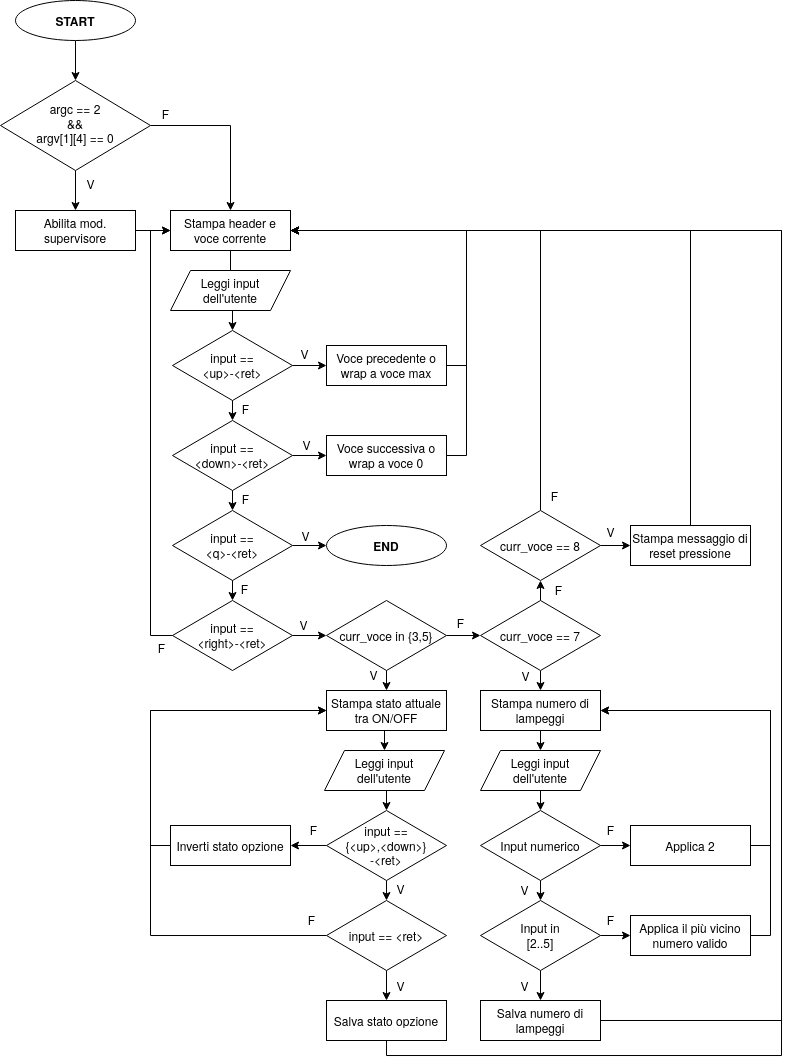
\includegraphics[height=17.8cm]{Flowchart auto_menu.drawio}
\end{center}

\chapter[nonumber=true]{Scelte progettuali}

L'implementazione del menù di configurazione dell'automobile descritta in queste pagine contiene alcune scelte progettuali operate con il fine di semplificare il codice sorgente, ridurre il codice duplicato e risparmiare memoria:

\begin{itemize}
\item L'impostazione grafica del menù è pensata per ricordare quanto più possibile quello (realmente esistente) della Lancia Ypsilon di II Generazione (tipo 843). Eccezion fatta per il menù di cambio del numero di lampeggiamenti, quindi, tutte le interfacce sono distribuite su due righe con l'header sulla superiore e l'inferiore dedicata a mostrare (a rotazione) le voci selezionate.
\item Il programma è pensato per gestire solo e soltanto gli input previsti dalle specifiche. Per quanto si sia tentato di gestire alcune eccezioni, non si garantisce il corretto funzionamento a fronte dell'inserimento di stringhe diverse da quelle esplicitamente supportate.
\item Il programma verifica il codice supervisore solo se questo viene passato senza altri parametri. Nel caso in cui venissero specificati più parametri il programma considererà automaticamente errato il codice inserito.
\item Il trasferimento dei parametri alle funzioni avviene mescolando registri e memoria, senza utilizzare uno standard preciso (per quanto il registro utilizzato sia sempre \texttt{\%eax} e la sezione di memoria sia sempre lo stack) ma ricorrendo alla tecnica migliore per ottimizzare le operazioni all'interno della funzione
\item Non essendo pensate per essere generali e riutilizzabili, le funzioni in questo progetto NON garantiscono che, una volta restituito il controllo al chiamante, i registri siano nello stato di partenza. Il compito di effettuare un backup dei valori indispensabili sullo stack è quindi lasciato al chiamante.
\item L'implementazione in C del programma non fa uso di \texttt{stdio} e di altre astrazioni normalmente utilizzate. Questo con lo scopo di calcare quanto più possibile il comportamento della versione Assembly, riducendo la distanza tra le due implementazioni per consentire di usare la versione C come una sorta di traduzione in linguaggio umano di quella Assembly.
\end{itemize}

\end{document}
